\section{Methodology}
\label{sec:method}
\subsection{ADNI Dataset}
The datasets used in the preparation of this article were obtained from the Alzheimer’s Disease Neuroimaging Initiative (ADNI) database \cite{lu_multimodal_2018}. The ADNI was launched in 2003 as a public-private partnership, led by Principal Investigator Michael W. Weiner, MD. The primary goal of ADNI has been to test whether serial magnetic resonance imaging (MRI), positron emission tomography (PET), other biological markers, and clinical and neuropsychological assessment can be combined to measure the progression of mild cognitive impairment (MCI) and early Alzheimer’s disease (AD). De-identified patient data was obtained and were placed into a server where the images could be accessed for pre-processing and use in the pipeline. The dataset used for AD Classification was obtained by the search criteria ADNI phase 1, Subjects: MCI, AD and CN, subjects with both PET and MRI (Axial) and chosen original images. In total there are 1006 images (450 MCI, 244 CN, and 312 AD) for 233 patients. In addition, we found that the MRI images from this dataset were masks and used a previously downloaded MRI with PET images from this dataset.   This hybrid dataset has 2102 images (1166 MCI, 515 CN, and 421 AD) for 290 patients.  

The dataset used for AD Progression was obtained by searching criteria ADNI, Subjects: MCI, AD and CN, modalities: subjects with PET or MRI. Then we filtered for subjects with both MRI and PET images such that the images have been through their preprocessing steps. For PET the preprocessing steps are co-registration, averaging, standardization of voxel sizes and uniforming the resolution.  The MRI preprocessing steps are intensity normalization and scaling. This dataset has 3177 images. Then the subjects’ images were divided into 7 timepoints based on their visit label and if from one timepoint to the next their diagnosis label didn’t change, a new label of stable MCI (sMCI) were created for them, otherwise if their diagnosis had changed, they got the new label of progressive MCI (pMCI). There are 521 sMCI and 466 pMCI

\subsection{AD Classification}
\begin{figure}
    \centering
    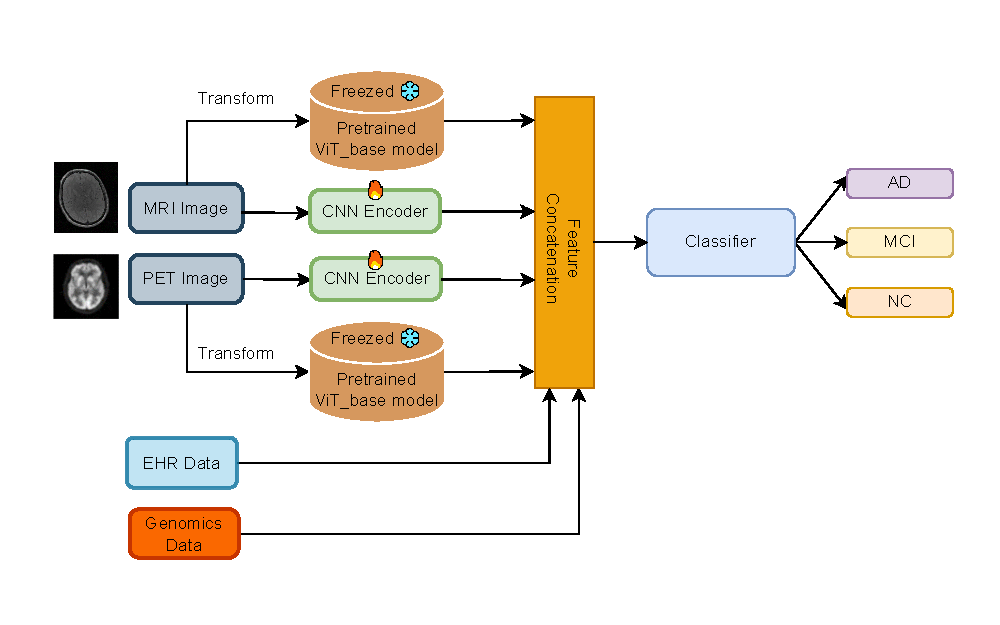
\includegraphics[width=1\linewidth]{figs/arch-classification_new.pdf}
    % \vspace{-2mm}
    
    \caption{Proposed architecture for multimodal AD classification}
    \vspace{-2mm}
    \label{fig:enter-label}
\end{figure}
In this study, we propose a novel classification method for AD that utilizes CNN and vision transformer (ViT\cite{dosovitskiy_image_2021}) to extract features of each modality and combine them for AD classification. The method combines two imaging modalities: MRI and PET. The architecture of our model is shown in Figure 1. For each modality (MRI and PET), the feature extraction with CNN is a custom architecture consisting of two convolution layers with ReLU and pooling. Then, we use the pre-trained ViT model to capture global and long-range dependencies. The preprocessing includes reshaping the 3D image data and select the first channel to adapt to the ViT input format, and then extract the features. 

Next, we did feature fusion using concatenation and multiplicative methods. The concatenation method combines the MRI and PET features from CNN and ViT together to form a combined feature representation. This combined feature then passes through two fully connected layers, and finally outputs the AD classification result (AD, MCI or NC). During the training process, the entire model is optimized in an end-to-end manner. 

The AD Progression pipeline consists of dividing the subjects’ visits into 7 timepoint pairs (t to t+1). The feature extraction for MRI and PET were done using either a pretrained convolutional neural net (CNN, ResNet18) or a pretrained Vision Transformer (ViT, vit-base-patch16-224). The feature extraction for EHR sex was done by converting it to 0 (female) or 1 (male), and for age it was normalized to values from 0 to 1. The Genetic data used is the Polygenic Hazard Score (PHS) which is a score based on APOE and 31 other genetic variants \cite{desikan_genetic_2017}. The PHS was normalized from 0 to 1. The next step is Feature Fusion where the PHS and along with EHR (sex and age), PET (1000 features) and MRI (1000 features) were combined in a feature matrix such that each subject had 2003 features. Then we did dimensionality reduction using Principal Component Analysis (PCA) and then we did the classification using Support Vector Machine with linear kernel.  

The dataset for each timepoint was then split into training and testing using a 5-fold cross-validation (80:20 train-test split). The hyperparameter optimization was done on different number of components for PCA: 2, 10, 25 and different number of components for the SVM classifier: 1, 10, 50. 

The hybrid model architecture for the AD progression , named BrainModel, integrates a pre-trained ResNet18 convolutional neural network (CNN) and a Vision Transformer (ViT) to leverage the strengths of both architectures for image classification tasks. The ResNet18 model is utilized for its robust feature extraction capabilities from convolutional operations, with its final fully connected layer removed and replaced by an identity layer to extract features. The ResNet18 layers are partially frozen, allowing only the parameters in the last convolutional block (layer4) to be trainable, ensuring the early layers' learned representations remain intact while allowing adaptation of higher-level features.

Parallel to the ResNet18, the ViT model is employed to capture global context and spatial relationships in the image. The ViT is also pre-trained, with the early layers frozen and only the last two blocks' parameters set as trainable, enabling fine-tuning of the model to the specific task at hand. Features from both models are extracted and concatenated, forming a combined feature vector comprising 512 features from ResNet18 and 768 features from ViT.

This combined feature vector is then passed through a fully connected layer reducing the dimensionality to 256 features, followed by a dropout layer with a 50\% dropout rate to mitigate overfitting. The final layer is a fully connected layer that maps the 256 features to the target number of classes, which is 2 in this case. The overall architecture allows the model to harness the detailed local feature extraction of the CNN and the global context understanding of the ViT, resulting in a powerful hybrid model for image classification.

To enhance the performance and robustness of our hybrid model, we employed a two-stage transfer learning process using separate models for MRI and PET images. For the MRI images, we utilized the BrainModel architecture and performed transfer learning using the entire MRI dataset. This process involved fine-tuning the pre-trained ResNet18 and ViT models within the BrainModel, adjusting their trainable layers to the specific characteristics of MRI data. The refined MRI model, thus adapted, was subsequently used to extract high-level features from the MRI dataset, capturing both local and global patterns effectively.

Similarly, a separate BrainModel was employed for the PET images. This PET-specific BrainModel underwent transfer learning using the entire PET dataset, fine-tuning the pre-trained ResNet18 and ViT models to capture the unique attributes of PET data. The adapted PET model was then used to extract robust features from the PET images. These features, derived from separate MRI and PET models, were then combined in the hybrid model to leverage the complementary information from both imaging modalities.

The training process utilized a 10-fold cross-validation scheme to ensure robustness and generalization. This was achieved using the KFold class from scikit-learn, configured with 10 splits, shuffled data, and a fixed random state for reproducibility. The key hyperparameters for training included a learning rate of 0.001, a batch size of 4, and a total of 25 epochs. Additionally, a weight decay of 1e-4 was applied to regularize the model and prevent overfitting. This systematic approach ensured that the hybrid model was finely tuned and capable of effectively integrating the distinct features from MRI and PET images.

\subsection{Modality Contributions}
\textbf{AD Classification}
In this study, we explore the impact of various modalities on AD classification by employing different single and combined modalities. We utilized PET, MRI, EHR, and genomic data. Our methodology involves setting up distinct experimental conditions for each modality and combinations thereof, particularly focusing on MRI and PET due to their prevalent use in medical imaging. The multimodal model, combining MRI and PET, is further examined under various hyperparameter settings to gauge stability and effectiveness in AD classification. 

For in-depth learning the importance of different modality, we conduct feature permutation experiments in the multimodal ViT-CNN model to assess the individual contributions of each modality, we record the features of each different modality from different networks from the feature splicing layer (named mri-cnn, pet-cnn, mri-vit, pet-vit, ehr). To assess the importance of features from different modalities in AD classification, we employ the permutation importance method. First, we evaluate the trained model on the test set to obtain baseline accuracy. Then, for each feature in the CNN and ViT components of both MRI and PET modalities, we perform multiple iterations of feature permutation. In each iteration, we randomly shuffle the values of a single feature while keeping other features unchanged, and re-evaluate the model's accuracy on the test set. The difference between the permuted accuracy and the baseline accuracy is calculated as the importance score for that feature. Finally, we average the importance scores across all iterations to obtain the final importance measure for each feature. 

\textbf{AD Progression}
One important question in Multimodal AD classification and prediction is how much each modality is contributing to the classifications. This was tested for the AD Progression by just doing the classification based on features extracted from CNN vs. ViT from MRI, PET, MRI \& PET, EHR \& Genetic, and MRI \& PET \& EHR \& Genetic.
\begin{figure}
    \centering
    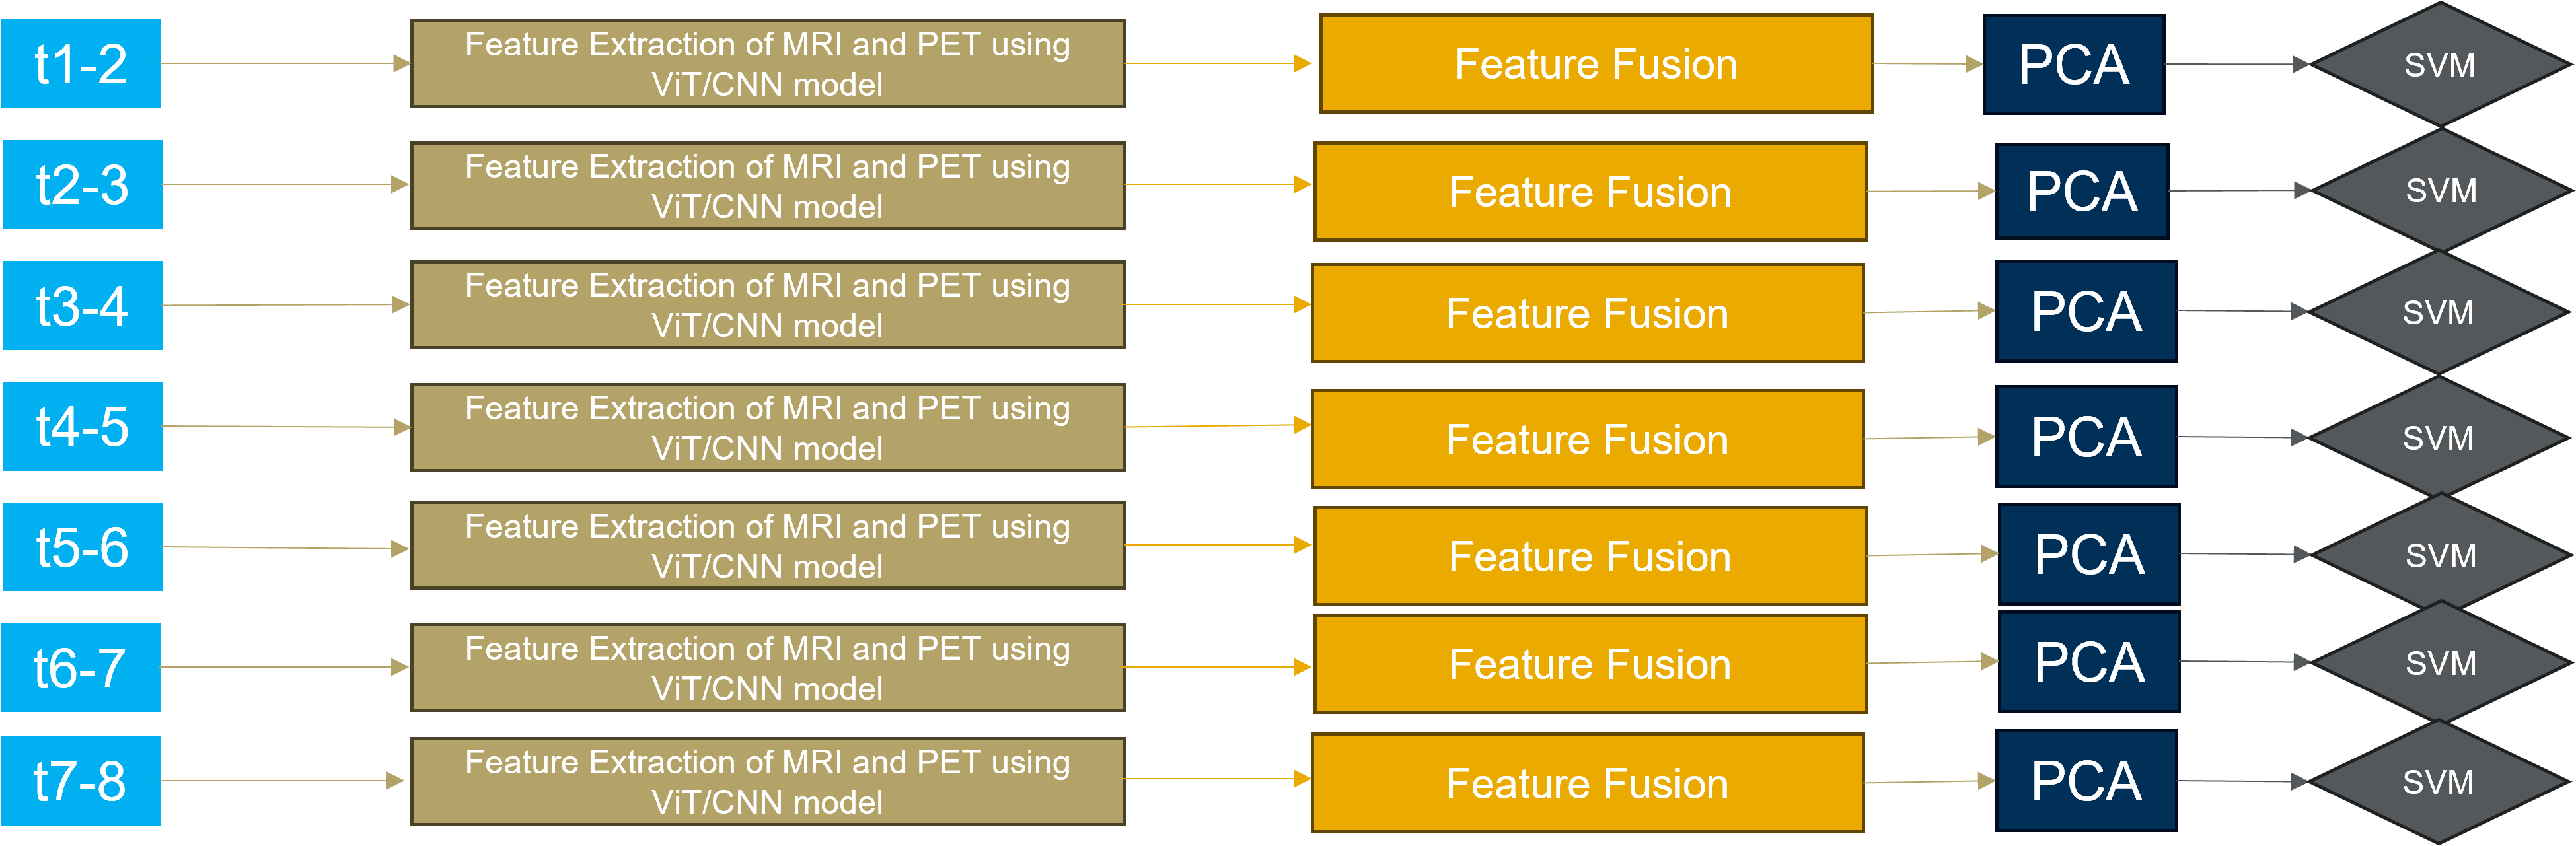
\includegraphics[width=1\linewidth]{figs/Picture14.png}
    \caption{Proposed architecture for multimodal AD Progression }
    \label{fig:enter-label}
\end{figure}